\documentclass[a4paper, 12pt]{report}

\usepackage[spanish]{babel}
\usepackage[utf8]{inputenc}
\usepackage[left=4cm, right=4cm, top=4cm]{geometry}
\usepackage{textcomp}
\usepackage{booktabs}
\usepackage{amssymb}
\usepackage{bussproofs}
\usepackage{fancyhdr}
\usepackage{graphicx}
\usepackage{amsmath}
\usepackage{enumitem}
\usepackage{ifsym}


\usepackage{hyperref}
\hypersetup{
    colorlinks=true,
    linkcolor=blue,
    filecolor=magenta,
    urlcolor=cyan,
}

\pagestyle{fancy}
\lhead{Almeida, Figueroa \& Ibarra}
\chead{Tarea 4}
\rhead{\today}

\begin{document}
\begin{titlepage}
    \centering
    {\scshape\Huge Universidad Nacional Autónoma de México \par}
    \vspace{1.25cm}
    {\scshape\huge Fundamentos de Bases de Datos\par}
    \vspace{1.25cm}
    {\huge\bfseries Tarea 4: Álgebra Relacional\par}
    \vspace{1.25cm}
    {\Large\textsc Almeida Rodríguez Jerónimo\par}
    \vspace{.1cm}
    {\large\texttt{418003815}\par}
    \vspace{0.25cm}
    {\Large\textsc Figueroa Sandoval Gerardo Emiliano\par}
    \vspace{.1cm}
    {\large\texttt{315241774}\par}
    \vspace{0.25cm}
    {\Large\textsc Ibarra Moreno Gisselle \par}
    \vspace{.1cm}
    {\large\texttt{315602193}\par}
    \vspace{1.5cm}
    \vfill
    \begin{figure}[hb!]
        
\includegraphics[width=.3\textwidth]
            {../logos/escudo_f-ciencias.png}\hfill
        
\includegraphics[width=.3\textwidth]
            {../logos/Escudo_UNAM.png}\hfill
    \end{figure}
\end{titlepage}

\section*{Ejercicio 1}{
\begin{enumerate}[label=\alph*)]
\item{Toda la información de los usuarios que tienen una página, pero no
        incluyen blog.\\
    $r = \pi$ user,  pagina, titulo\_blog (Usuario $\Join$ Página $\Join$ Blog)\\
    $p = $ user $\gamma$ count(pagina) $\rightarrow$ num\_p (r)\\
    $b = $ user $\gamma$ count(titulo\_blog) $\rightarrow$ num\_b (r)\\
    $Q = p \Join b$\\
    $t =pi$ user ($\sigma$ num\_b $= 0 \wedge$ num\_p$ > 0$ ($Q$))\\
    $pi *$ (User $\Join$ t)
    }
\item{}
\item{}
\item{Jero}
\item{}
\end{enumerate}
}

\section*{Ejercicio 2}{
\begin{enumerate}[label=\alph*)]
\item{}
\item{¿Qué fabricantes producen computadoras portátiles con un disco duro de
    menos 100 GB?\\
    \begin{figure}[hb!]
        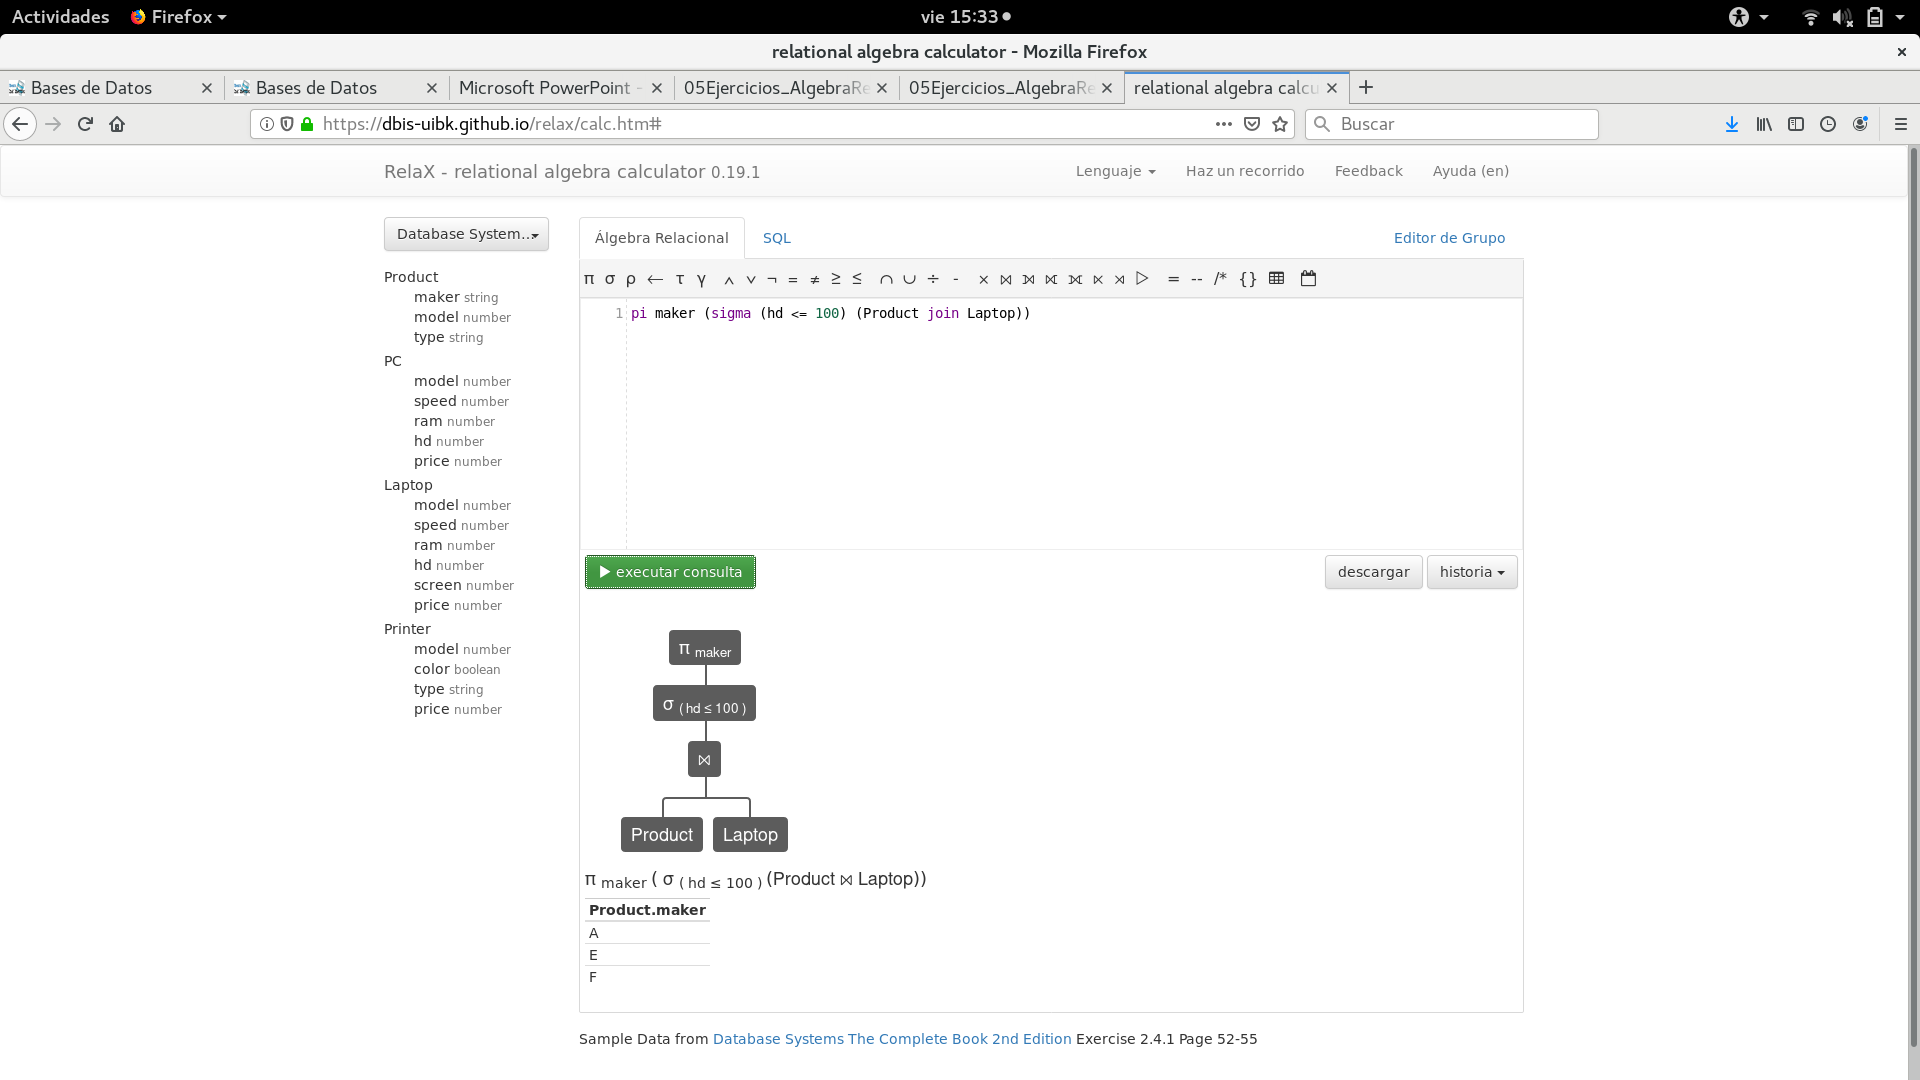
\includegraphics[width=\textwidth]
            {img/b.png}\hfill
    \end{figure}
}
\item{r = $\sigma$ fabricante = 'B' (Producto)\\
	s = $\pi$ modelo, precio (Laptop) $\cup$ $\pi$ modelo, precio (PC)
	$\cup$ $\pi$ modelo, precio (Impresora) \\
	$\pi$ modelo, precio (s $\Join$ r)}
\item{}
\item{Encontrar los números de modelo de todas las impresoras láser a color.\\
    \begin{figure}[hb!]
        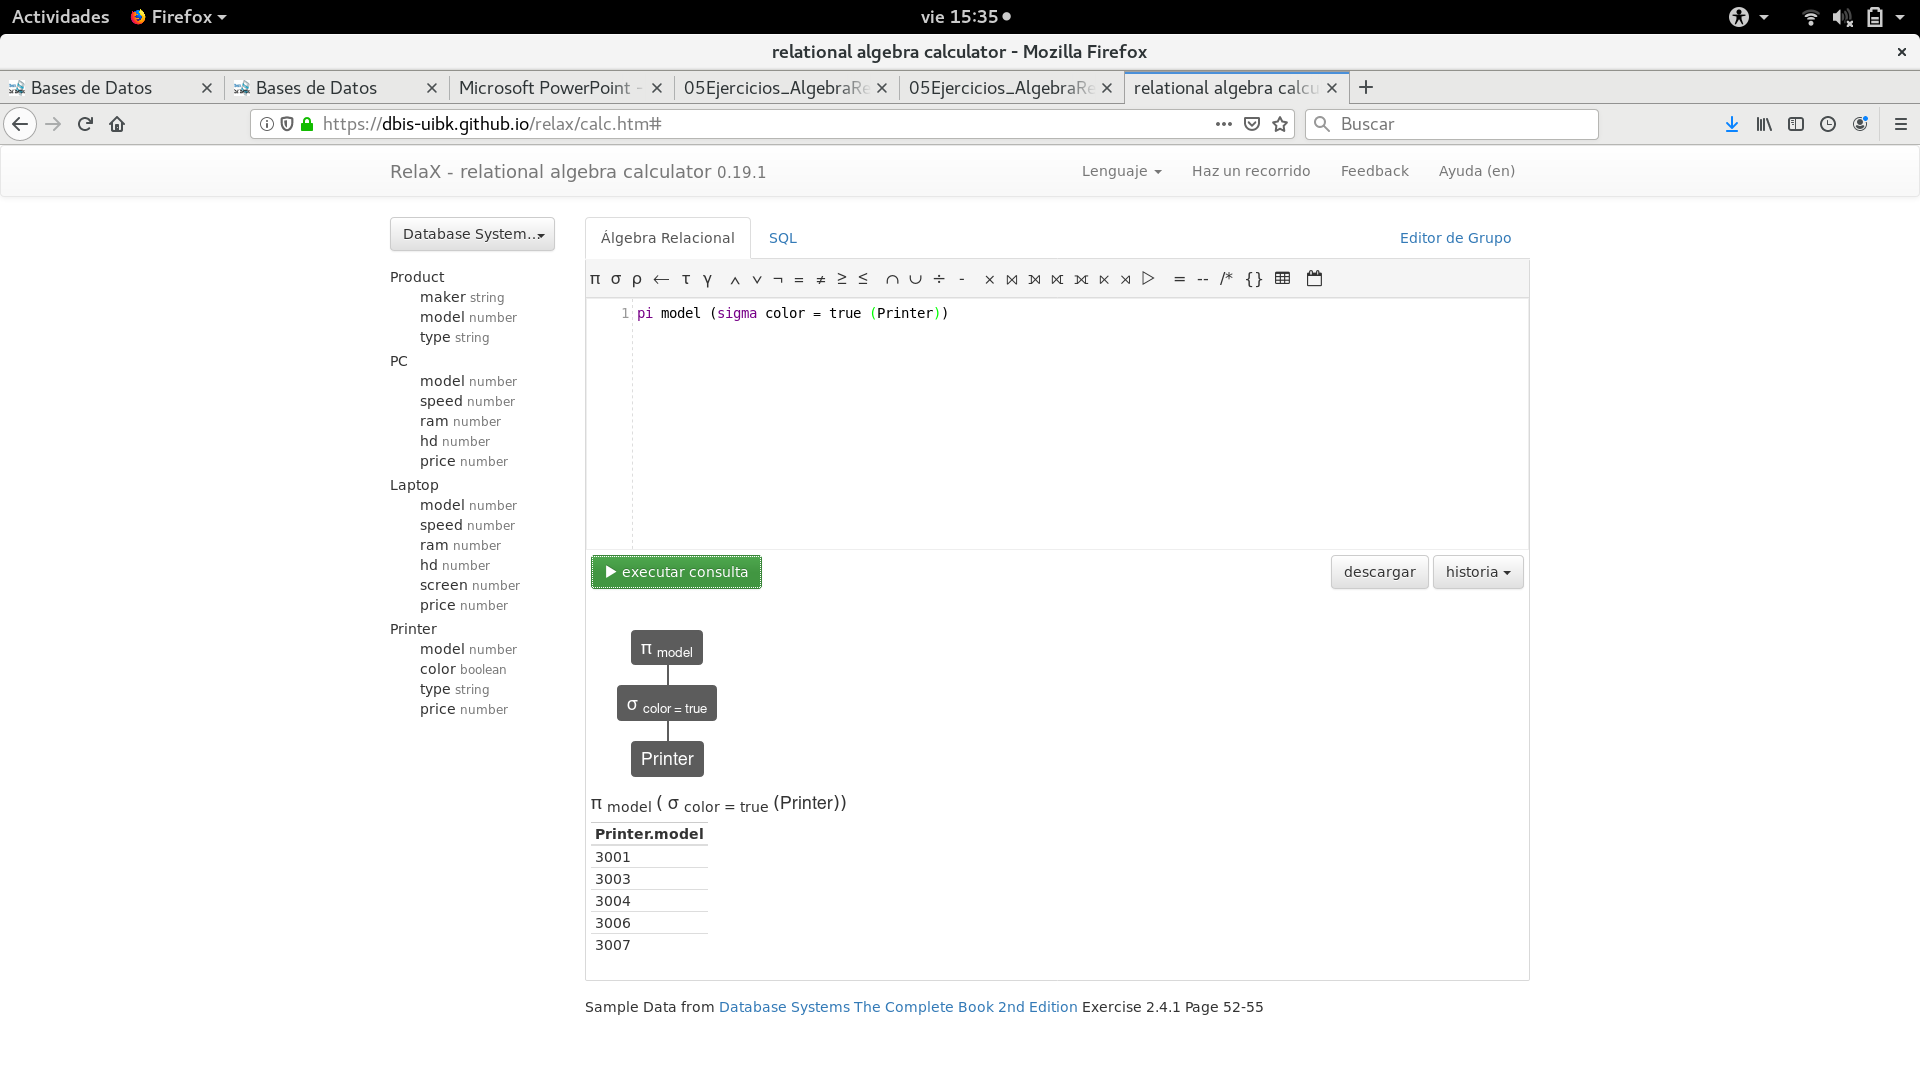
\includegraphics[width=\textwidth]
            {img/e.png}\hfill
    \end{figure}
}
\item{r = $\pi$ modelo, fabricante (Producto)\\
	s = $\pi$ fabricante ($\pi$ modelo (Laptop) $\Join$ r)\\
	t = $\pi$ fabricante ($\pi$ modelo (PC) $\Join$ r)\\
	s - t\\}
\item{}
\item{Encontrar toda la información de las PCs que tienen la misma velocidad y
    RAM.\\
    \begin{figure}[hb!]
        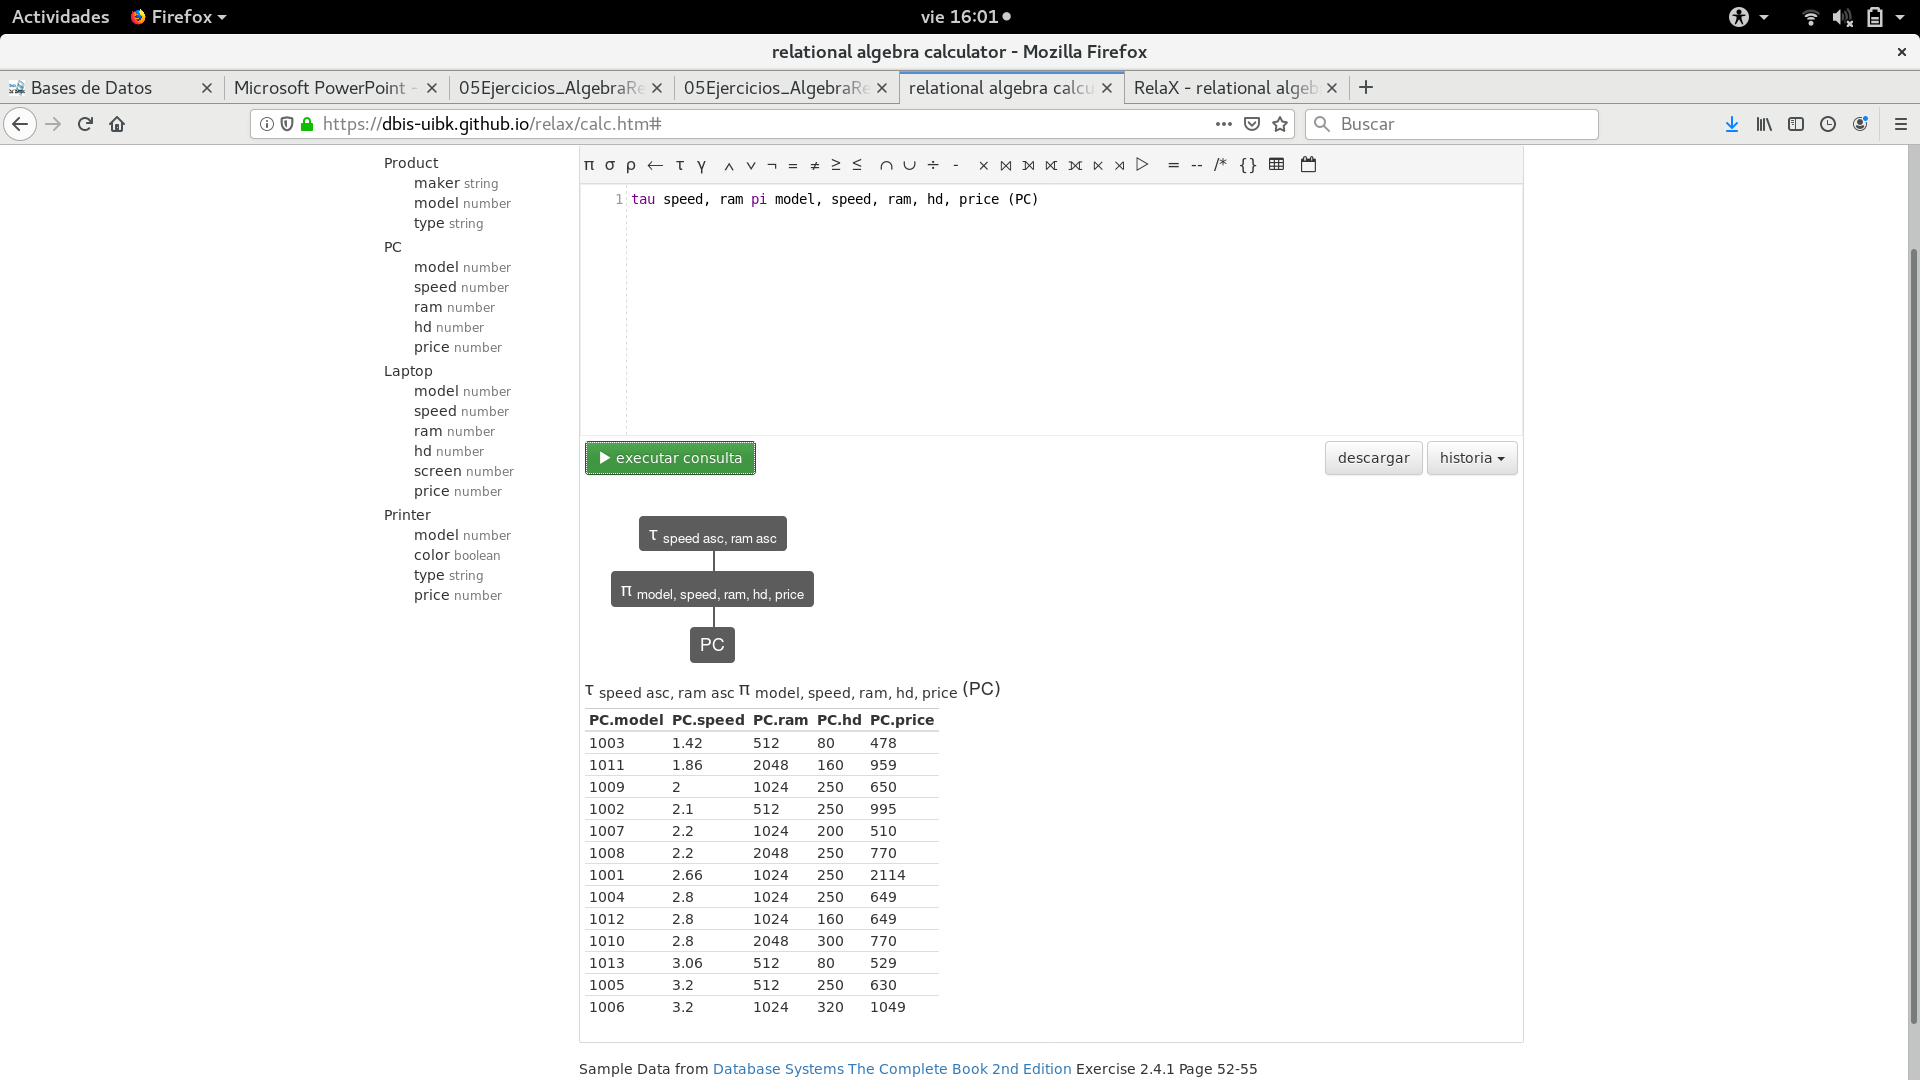
\includegraphics[width=\textwidth]
            {img/h.png}\hfill
    \end{figure}
}
\item{r = $\pi$ modelo ($\sigma$ velocidad $\geq$ 2.8 (PC))\\
s = $\pi$ modelo($\sigma$ velocidad $\geq$ 2.8 (Laptop))\\
$\pi$ fabricante ((r $\cup$ s) $\Join$ Producto)\\
}
\item{}
\item{Encontrar los fabricantes de PC con al menos tres velocidades diferentes.\\
    \begin{figure}[hb!]
        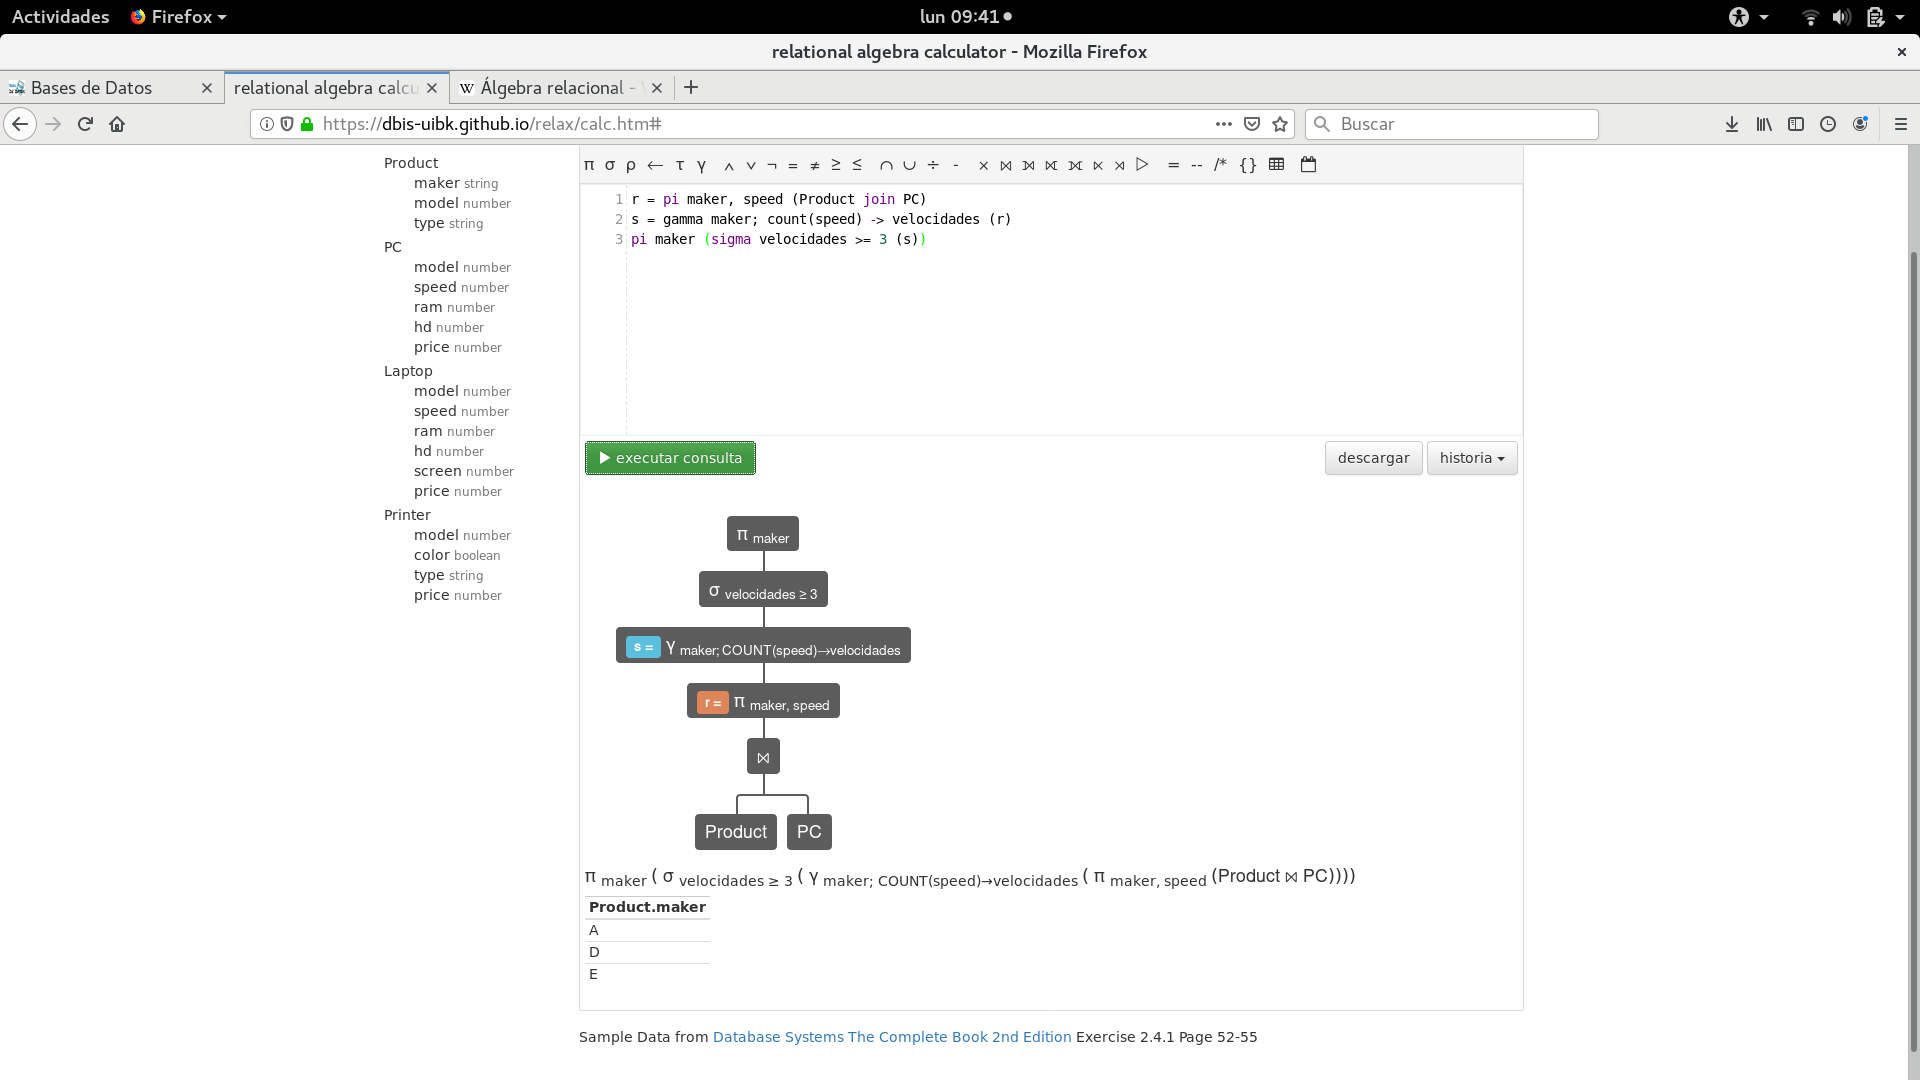
\includegraphics[width=\textwidth]
            {img/k.png}\hfill
    \end{figure}
}
\item{r = $\pi$ modelo, fabricante (Producto $\Join$ PC)\\
s = Y fabricante; count(modelo) $\rightarrow$ numproductos (r)\\
$\pi$ fabricante ($\sigma$ numproductos = 3 (s))}
\item{}
\item{Crear un reporte que muestre por fabricante, el número de productos que tiene de cada tipo.\\
    \begin{figure}[hb!]
        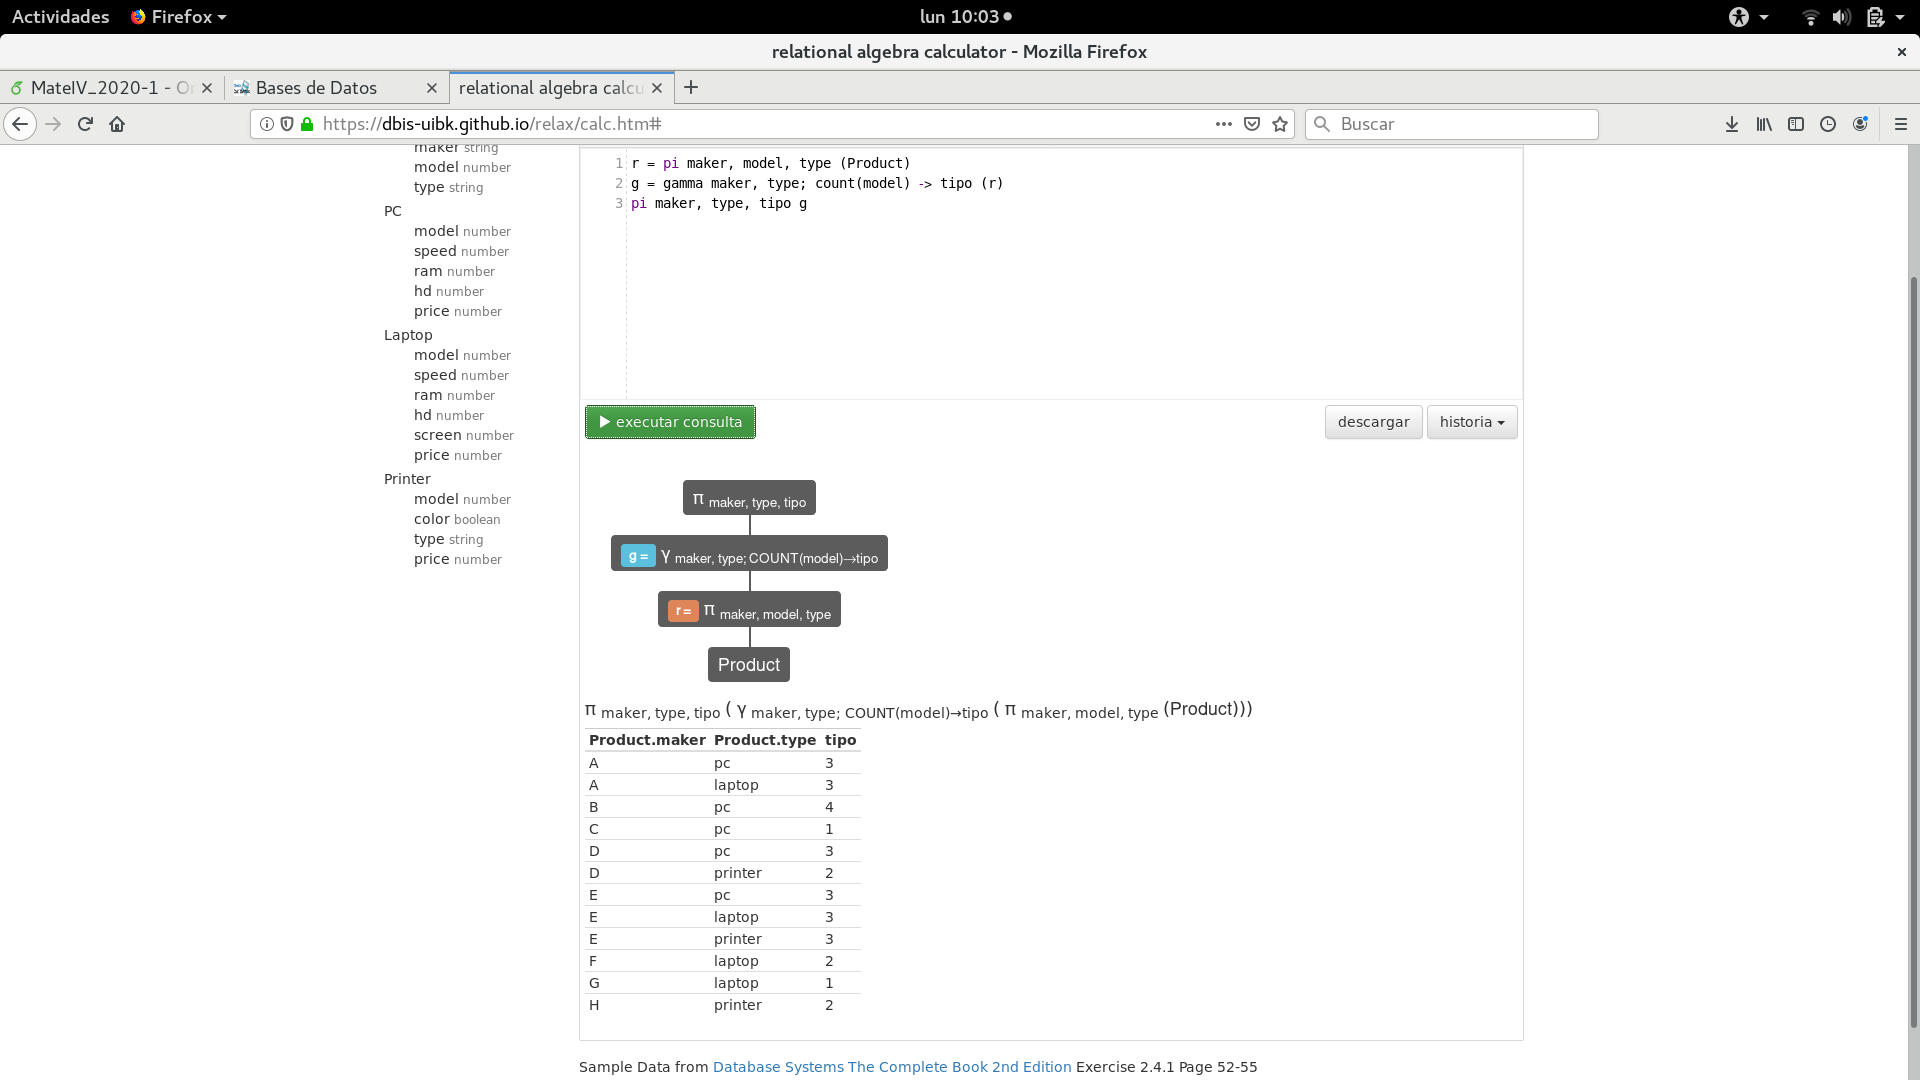
\includegraphics[width=\textwidth]
            {img/n.png}\hfill
    \end{figure}
}
\item{r = $\pi$ modelo ($\sigma$ fabricante = 'E' (Producto)) $\Join$ Laptop\\
s = $\sigma$ hd $<$ 200 (r)\\
t = $\pi$ modelo, velocidad, ram, hd\_nuevo $\leftarrow$ hd * 1.15, pantalla, precio (s)\\
t}
\item{}
\item{Jero}
\item{}
\end{enumerate}
}



\end{document}
